\begin{table}[h]
    \centering
    \caption{Comparação do Tempo do HeapSort}
    \begin{tabular}{|c|c|c|c|c|c|c|}
        \hline
        Tamanho de Entrada & 10 & 100 & 1000 & 10000 & 100000 & 1000000 \\
        \hline
        Crescente & 0.000000 & 0.000000 & 0.000000 & 0.002000 & 0.018000 & 0.212000 \\
        \hline
        Decrescente & 0.000000 & 0.000000 & 0.000000 & 0.002000 & 0.018000 & 0.215000 \\
        \hline
        Aleatória & 0.000000 & 0.000000 & 0.000000 & 0.001000 & 0.023000 & 0.318000 \\
        \hline
    \end{tabular}
    \label{tab:comparacaobubble}
\end{table}

A tabela apresenta a performance do algoritmo Heap Sort em seis diferentes tamanhos de entrada e em três situações distintas de ordenação dos dados: crescente, decrescente e aleatória. Os resultados demonstram as características notáveis do Heap Sort, um algoritmo eficiente para criar uma estrutura de dados de heap e realizar a ordenação.

Observa-se que, para entradas de pequeno tamanho (10 e 100), o tempo de execução é insignificante, refletindo a eficiência do algoritmo em lidar com conjuntos de dados menores. À medida que o tamanho da entrada aumenta, nota-se um crescimento gradual no tempo de execução, o que é esperado dada a complexidade de tempo O(n log n) do Heap Sort.

As variações entre os tempos para entradas crescentes, decrescentes e aleatórias são mínimas, indicando que o Heap Sort não é sensivelmente afetado pela ordenação inicial dos dados. Isso contrasta com algoritmos como o Bubble Sort, que pode ter um desempenho pior em entradas decrescentes.

O Heap Sort mostra-se, portanto, como um algoritmo robusto e confiável, com bom desempenho consistente em diferentes cenários. Sua capacidade de manter uma performance estável o torna uma opção viável para aplicações onde os dados podem ser apresentados em qualquer ordem e onde o tempo de execução previsível é crítico.

 \begin{figure}[H]
    \centering
    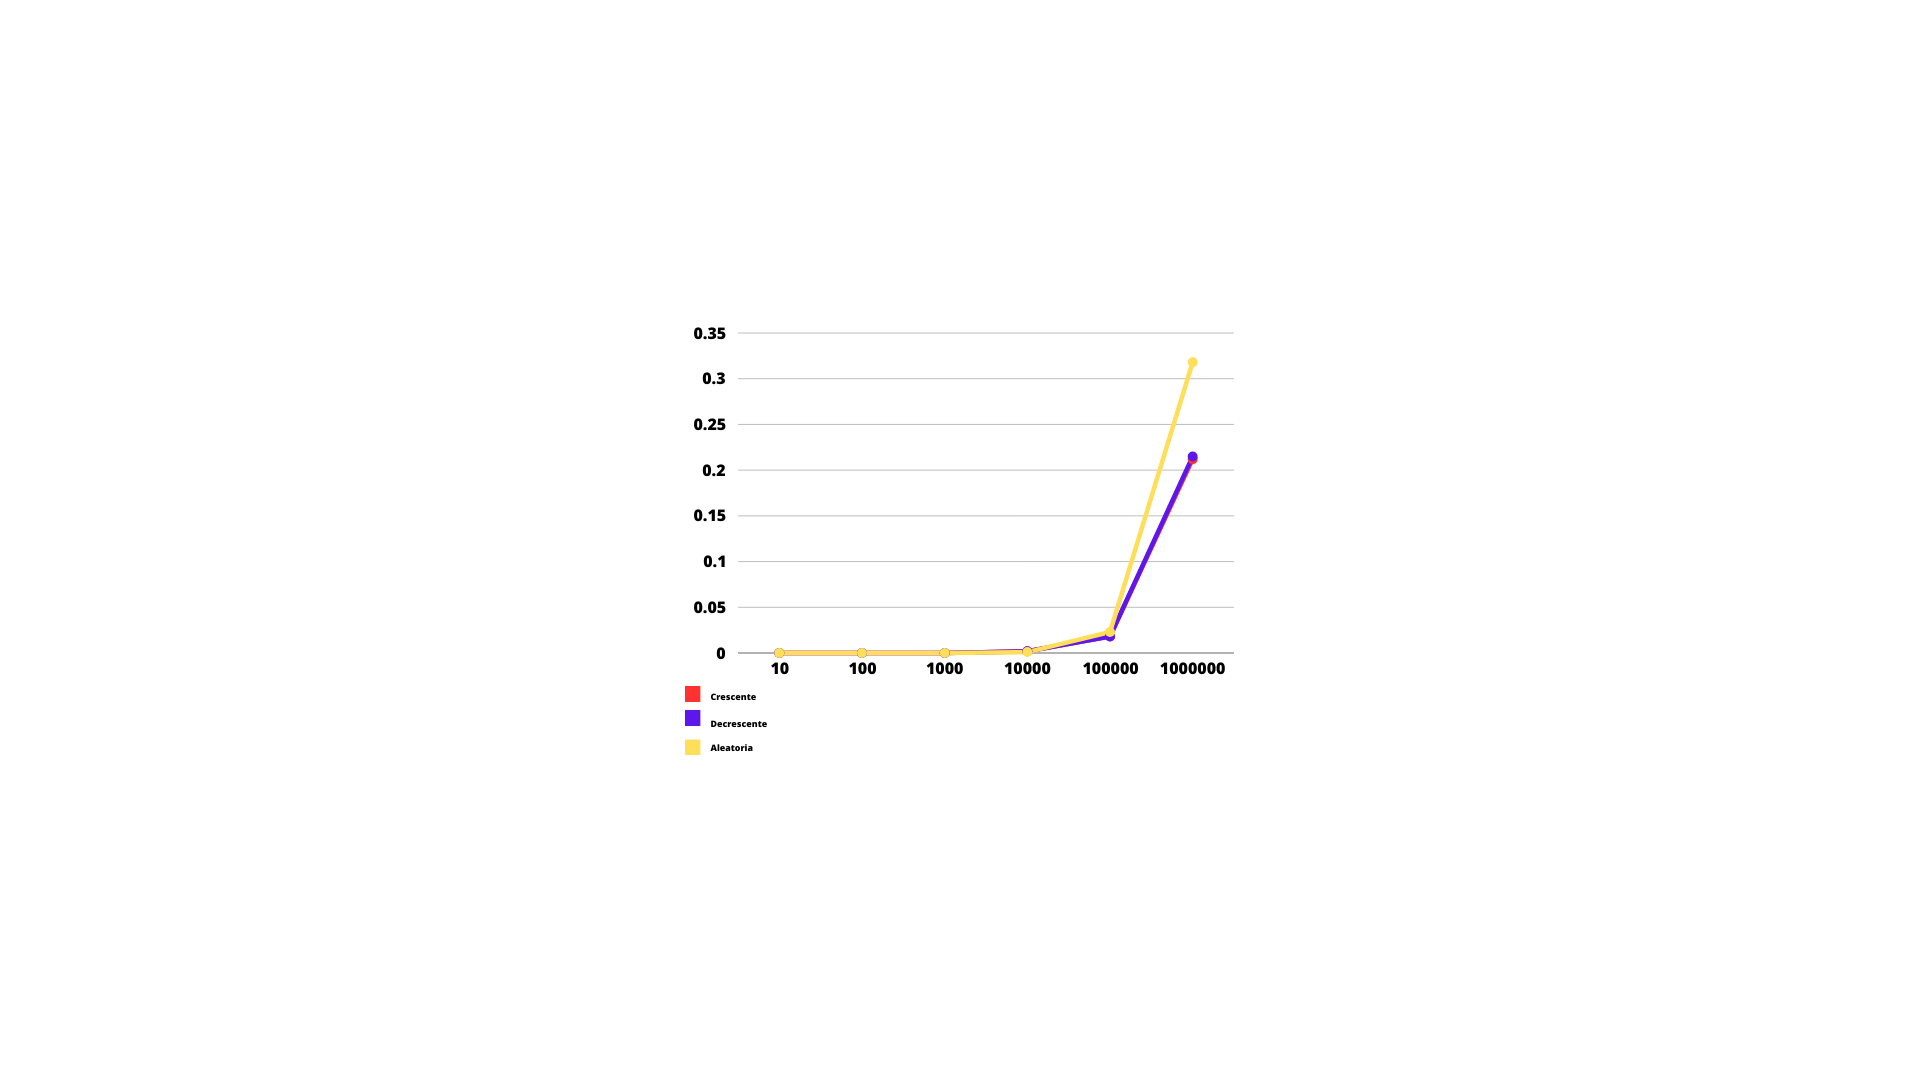
\includegraphics[width = 20cm]{Imagens/Heap Sort/zz.png}
    \caption{Gráfico de tempo do HeapSort. }
    \label{imagem_digrama}
\end{figure}
